\section{Background}
The relationship between input discharge (both water and sediment) and the resulting channel properties such as the channel width-to-depth ratio is unknown for the DeltaRCM model. 

\section{Model Runs}
A set of 7 model runs, each with a different input discharge are conducted by modifying the depth of the inlet, which alters the discharge fed into the domain without increasing the inlet width.
These runs are at ``field-scale" using parameters similar to those from previous studies \cite{Liang2016, Liang2016a}.
The YAML below provides information about the parameter set used.\\

\noindent \texttt{YAML} configuration file: \vspace{-6pt}
\begin{boxedverbatim}
timesteps: 5000
Length: 10000.0
Width: 22000.0
L0_meters: 150.0  # will be 3 cells (the minimum)
N0_meters: 250.0
hb: 5.0
dx: 100.0
SLR: 36e-10  # small background SLR
Np_water: 2000
Np_sed: 2000
save_dt: 250000

matrix:
  h0:
    - 4.0  # shallower than basin
    - 5.0  # same as basin
    - 6.0
    - 7.0
    - 8.0
    - 9.0
    - 10.0  # double basin
\end{boxedverbatim}

\section{Results}

\begin{figure}[!ht]
	\makebox[\textwidth][c]{
	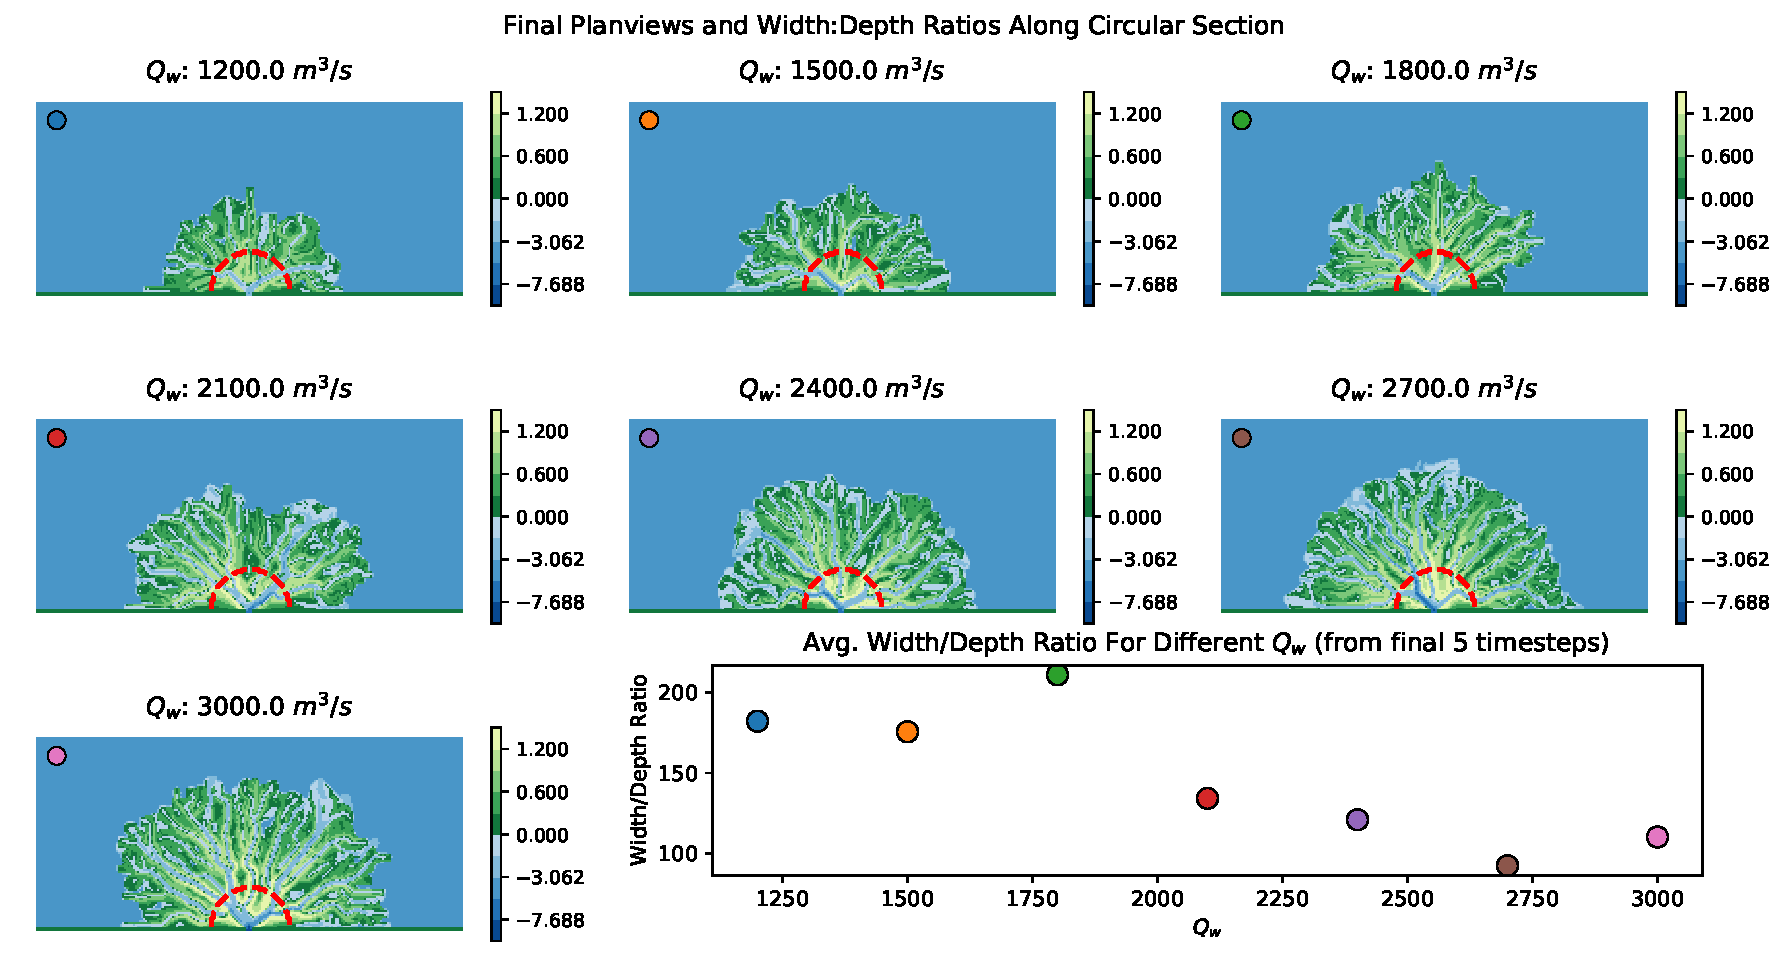
\includegraphics[width=\textwidth]{QandWidthDepth/figs/FinalPlans_WidthDepth.pdf}
	}	
	\caption{Final model topographies from the 7 runs generated by the YAML configuration file. Bottom right plot shows the average width-to-depth ratios of the channels along the circular sections shown in red, using data from the last 5 timesteps of each run.}
	\label{fig:QWD_plot}
\end{figure}

\section{Conclusions}
Unsurprisingly as the input discharge value is increased the size of the resulting delta increases. There is also an observed decrease in the width-to-depth ratios of the channels as the inlet discharge increases. 

\bibliographystyle{plainnat}
\bibliography{bib/bib}